\documentclass[a4paper, twocolumn]{article}
\usepackage{authblk}
\usepackage[font=small,labelfont=bf]{caption}
\usepackage{biblatex}
\addbibresource{references.bib}
\usepackage{lineno}
\usepackage{amsmath}
\usepackage{amsfonts}
\usepackage{tikz}
\usepackage{tkz-graph}
\usepackage{mathtools}
\usepackage{tabularx}
\usepackage{graphicx}
\usepackage{blkarray}
\usepackage{booktabs} 
\graphicspath{ {./figures/} }


\title{Optimal threshold problem: A novel 0-1 ILP-based approach}
\date{}
\author[1]{Pouria Ramazi}
\author[2]{Arash Mari Oriyad}
\affil[1]{Department of Mathematics and Statistics, Brock University, St. Catharines, L2S 3A1, ON, Canada}
\affil[2]{Department of Electrical and Computer Engineering, Isfahan University of Technology, Isfahan 84156-83111, Iran}
\setcounter{Maxaffil}{0}
\renewcommand\Affilfont{\small}

\usepackage[utf8]{inputenc}
\usepackage{fourier, heuristica}
\usepackage[colorlinks=true]{hyperref}
\usepackage{array, ltablex, multirow}

\usepackage{makecell}
\setcellgapes{5pt}
\makegapedcells
\renewcommand\theadfont{\bfseries}
\renewcommand\cellalign{rc}


\begin{document}
\maketitle
\linenumbers


%\begin{abstract}
%Abstract ... 
%\end{abstract}

Accuracy \cite{accuracy}, recall \cite{recall}, and specificity \cite{specificity} are three of the most used measures to evaluate binary classification models. Considering $TP$, $TN$, $FP$, and $FN$ as the number of true-positive, true-negative, false-positive, and false-negative instances, respectively, these measures can be calculated as follows:

\begin{equation}
\label{formulation_1}
\begin{aligned}
&accuracy = \frac{TP + TN}{TP + TN + FP + FN}\\
&recall = \frac{TP}{TP + FN}\\
&specificity=\frac{TN}{TN + FP}
\end{aligned}
\end{equation}

While calculating performance measures introduced in equation \ref{formulation_1} require deterministic labels, classification models often produce probabilistic outputs. Hence, one must apply a threshold to the probabilities generated by a classifier to obtain deterministic labels. An optimal accuracy (resp. recall and specificity) threshold for a given set of instances is a real value between 0 and 1, resulting in the highest accuracy (resp. recall and specificity).

A trivial approach to determine such a threshold is an exhaustive search over all possible thresholds to obtain the best one. As an alternative method, we introduce a 0-1 ILP formulation for finding the optimal threshold for accuracy, recall, specificity, and any linear combination of them.

Assume a set of $N$ instances with a binary target variable $y$. We call $N^+$ and $N^-$ as the number of positive and negative instances. Also, suppose $\hat{y_i}$ is the probability predicted by a classifier for the $i$th instance. Then, $\tilde{y_i}$ would be a binary decision variable that represents the label of $i$th instance after applying the threshold $t$ to $\hat{y_i}$ and can be calculated as below.

\begin{equation}
\label{y_tilde_formulation}
\begin{aligned}
\tilde{y_i} = 
\begin{cases}
0, & \hat{y_i} < t \\
1, & \hat{y_i} \ge t
\end{cases}
\end{aligned}
\end{equation}

Using the introduced notations and according to equation \ref{formulation_1}, accuracy, recall, and specificity can be calculated as follows:

\begin{equation}
\begin{aligned}
&accuracy = 1 - \frac{1}{N} \sum_{i=1}^{N} |y_i - \tilde{y_i}|\\
&recall = \frac{1}{N^+} \sum_{i=1}^{N} y_i \tilde{y_i}\\
&specificity = \frac{1}{N^-} \sum_{i=1}^{N} (1-y_i) (1-\tilde{y_i})\\
\end{aligned}
\end{equation}

Put them all together, the following optimization formulation is achieved to find the optimal threshold maximizing $\alpha \times \textit{accuracy} + \beta \times \textit{recall} + \gamma \times \textit{specificity}$, where $\alpha$, $\beta$, and $\gamma$ are the user-defined coefficients.

\begin{equation}
\label{optimization_formulation}
\begin{aligned}
	&\text{maximize} \quad \sum_{i=1}^{N} -\frac{\alpha}{N}|y_i -\tilde{y_i}| + \frac{\beta}{N^+} y_i \tilde{y_i} + \frac{\gamma}{N^-} (1-y_i) (1-\tilde{y_i})\\
	&\text{subject to:} \quad \tilde{y_i} = 
	\begin{cases}
	0, & \hat{y_i} < t \\
	1, & \hat{y_i} \ge t
	\end{cases} \qquad \forall 1\le i \le N\\
	& \qquad \qquad \qquad \tilde{y_i} \in \{0, 1\} \qquad \forall 1\le i \le N\\
	& \qquad \qquad \qquad 0 \le t \le 1 \qquad
\end{aligned}
\end{equation}

To make the objective function linear, we introduced new decision variable $z_i$ corresponding to the non-linear term $|y_i - \tilde{y_i}|$ along with 2 new constraints for each $i$ shown in equation \ref{ilp}. Moreover, to linearize $\tilde{y_i}$ constraints in equation \ref{optimization_formulation}, we combined the conditions and replace them with two new constraints for each $i$ in equation \ref{ilp}.

\begin{equation}
\label{ilp}
\begin{aligned}
&\text{maximize} \quad \sum_{i=1}^{N} -\frac{\alpha}{N}z_i + \frac{\beta}{N^+} y_i \tilde{y_i} + \frac{\gamma}{N^-} (1-y_i) (1-\tilde{y_i})\\
&\text{subject to:}\\
&\quad \: \: z_i \ge y_i - \tilde{y_i} \qquad \forall 1\le i \le N \qquad (1)\\
& \quad z_i \ge \tilde{y_i}  - y_i \qquad \forall 1\le i \le N \qquad (2)\\
& \quad \hat{y_i} (1 - \tilde{y_i}) < t \qquad \forall 1\le i \le N \qquad (3)\\
& \quad  \tilde{y_i} (\hat{y_i} - 1) \ge t - 1 \qquad \forall 1\le i \le N \qquad (4)\\
& \quad \tilde{y_i} \in \{0, 1\} \qquad \forall 1\le i \le N \\
& \quad z_i \in \mathbb{R} \qquad \forall 1\le i \le N \\
& \quad  0 \le t \le 1
\end{aligned}
\end{equation}

More precisely, constraints $(1)$ and $(2)$ force the decision variable $z_i$ to be greater than $|y_i - \tilde{y_i}|$. Hence, by maximizing $-z_i$, we are maximizing $-|y_i - \tilde{y_i}|$ too. Constraints $(3)$ and $(4)$ are formulating the relation between $\tilde{y_i}$ and $t$ represented in equation \ref{y_tilde_formulation}. For example, if $\hat{y_i} = 0.7$ and $t=0.5$ for an arbitrary $i$, then $\tilde{y_i}$ is forced to be $1$ according to the constraints $0.7 (1 - \tilde{y_i}) < 0.6$ and $\tilde{y_i} (0.7 - 1) \ge 0.6 - 1$.

Note that the proposed 0-1 ILP formulation in equation \ref{ilp} can not output $t=0$ as the optimal threshold and this case must be considered separately. 

To further improve the 0-1 ILP formulation, we considered a case where number of unique ordered pairs $(y_i,\: \hat{y_i})$ for $0 \le i \le N$ is significantly less than total number of instances, $N$. Suppose $M$ is the total number of distinct ordered pairs, and $m_i$ is the repetition number of a particular ordered pair in the original instance set. Hence, the following 0-1 ILP formulation is equivalence to the previous one but empirically more efficient.

\begin{equation}
\label{improved_ilp}
\begin{aligned}
&\text{maximize} \quad \sum_{i=1}^{M} m_i(-\frac{\alpha}{N}z_i + \frac{\beta}{N^+} y_i \tilde{y_i} + \frac{\gamma}{N^-} (1-y_i) (1-\tilde{y_i}))\\
&\text{subject to:}\\
&\quad \: \: z_i \ge y_i - \tilde{y_i} \qquad \forall 1\le i \le M \qquad\\
& \quad z_i \ge \tilde{y_i}  - y_i \qquad \forall 1\le i \le M \qquad\\
& \quad \hat{y_i} (1 - \tilde{y_i}) < t \qquad \forall 1\le i \le M \qquad\\
& \quad  \tilde{y_i} (\hat{y_i} - 1) \ge t - 1 \qquad \forall 1\le i \le M \qquad\\
& \quad \tilde{y_i} \in \{0, 1\} \qquad \forall 1\le i \le M \\
& \quad z_i \in \mathbb{R} \qquad \forall 1\le i \le M \\
& \quad  0 \le t \le 1
\end{aligned}
\end{equation}

The proposed 0-1 ILP formulation is compared with a search based method (Appendix 1) in terms of execution time (Fig. 1).
\begin{figure}[t]
	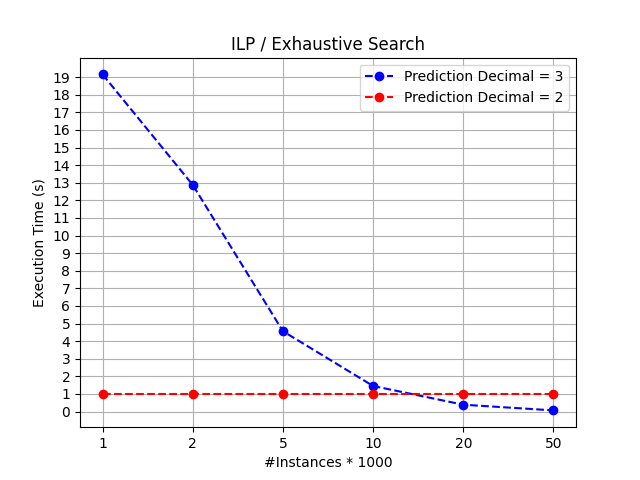
\includegraphics[width=\columnwidth]{figure_4_temp}
	\caption{Comparison between 0-1 ILP and exhaustive search methods in terms of average execution time. Each curve demonstrates the proportion of average execution time using the ILP approach respect to the search method. All experiments are repeated 100 times.}
\end{figure}

Conclusion/Discussion ...

\printbibliography

\end{document}
